\documentclass{standalone}
\usepackage{tikz}
\usetikzlibrary{patterns, positioning}
\usepackage[sfdefault]{ClearSans} %% option 'sfdefault' activates Clear Sans as the default text font
\usepackage[T1]{fontenc}

\begin{document}
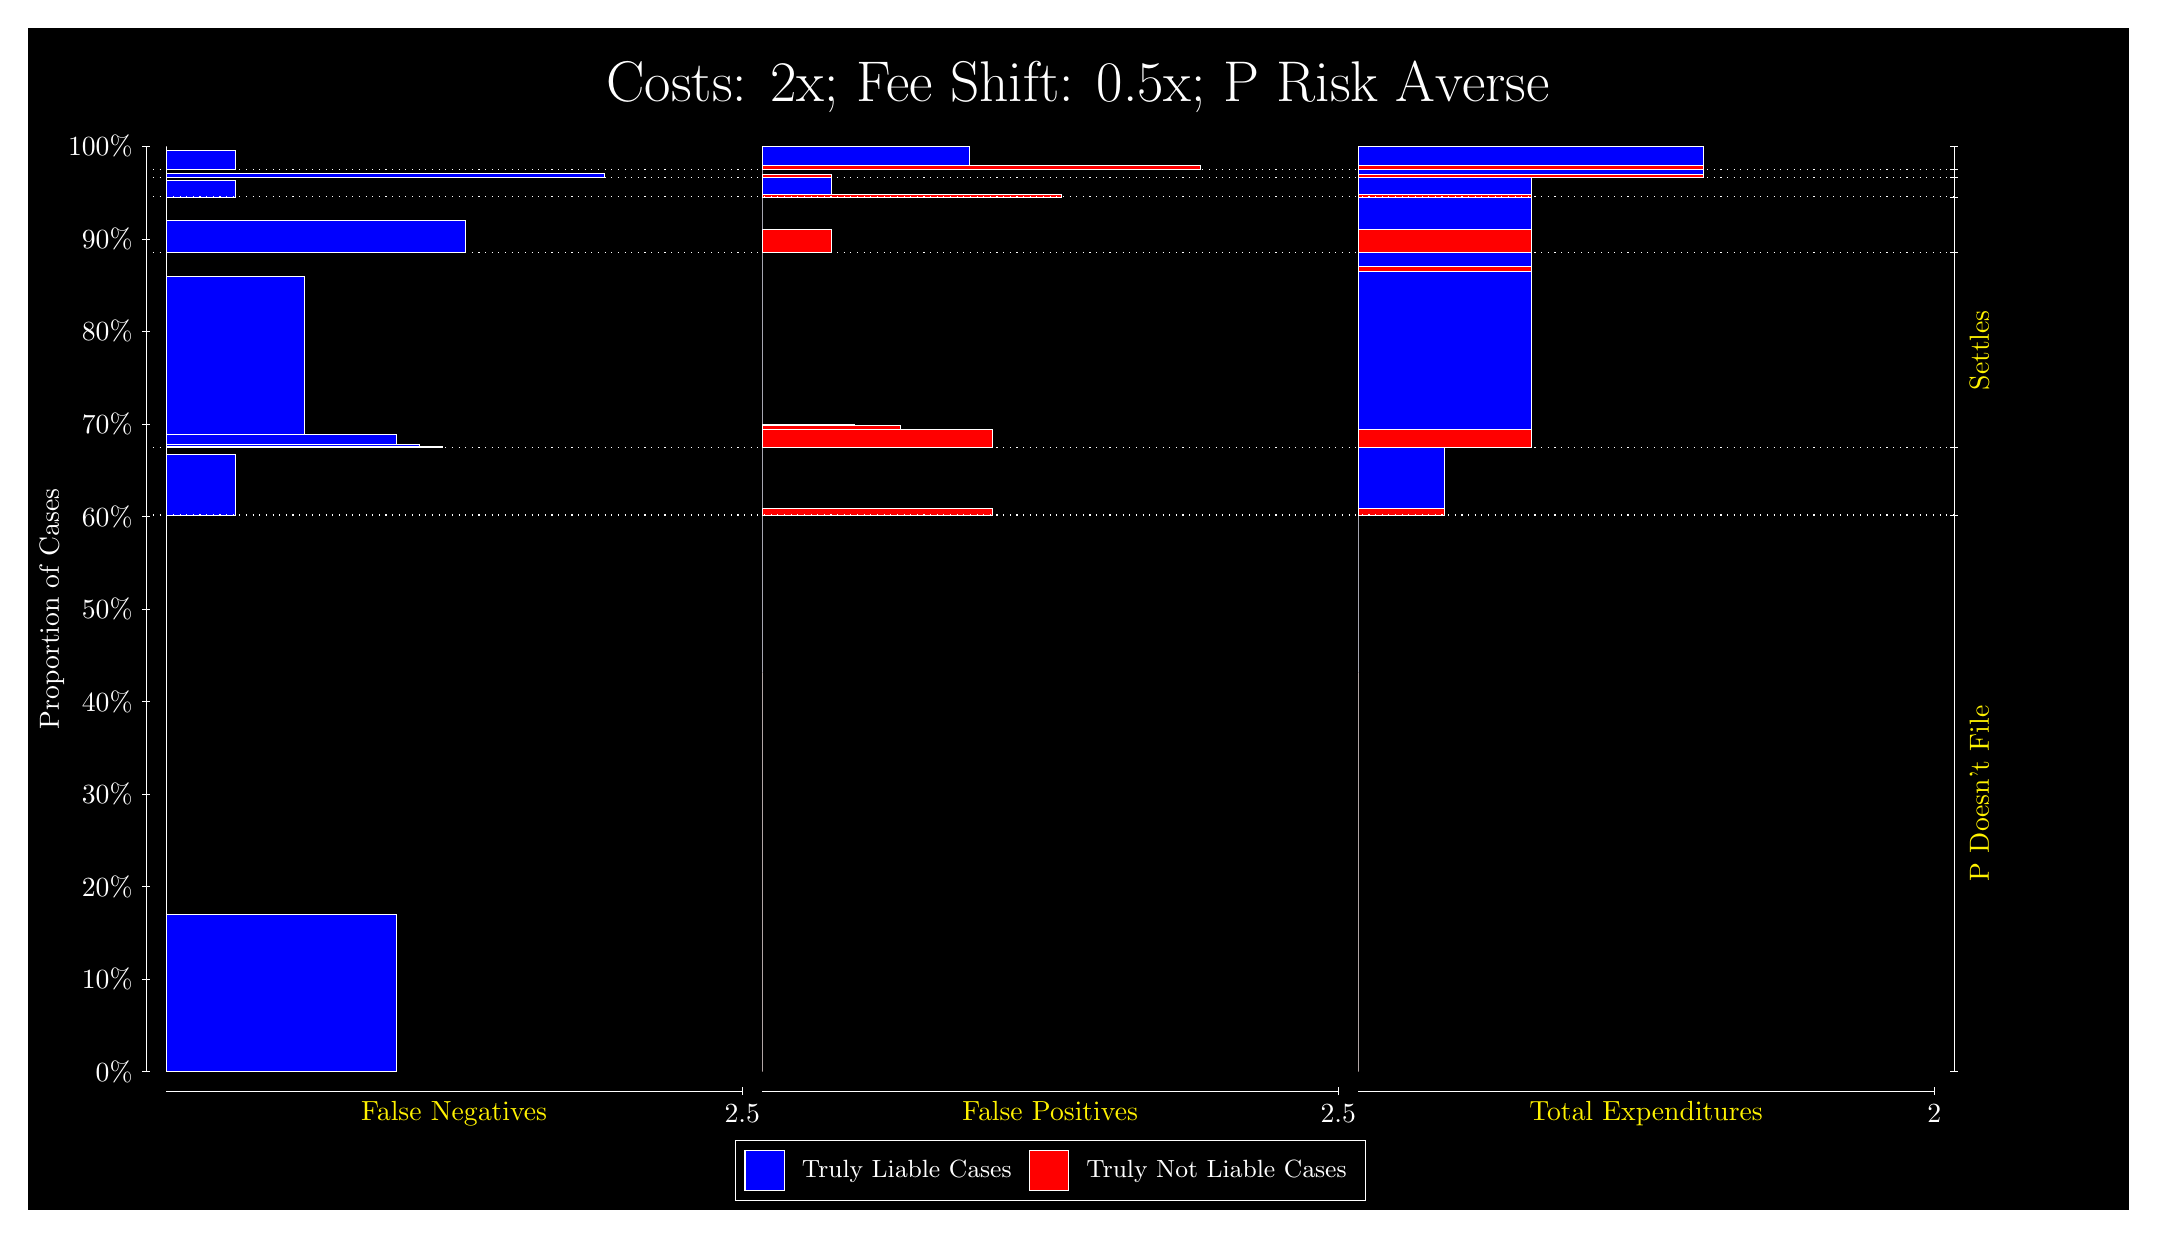
\begin{tikzpicture}
\draw[fill=black] (0,0) rectangle (26.667,15);
\draw[text=white] (0,13.5) rectangle (26.667,15) node[midway] {\huge Costs: 2x; Fee Shift: 0.5x; P Risk Averse};
\draw[white, very thin] (1.5,1.75) -- (1.5,13.5);
\node[rotate=90, text=white, anchor=center] at (0.3, 7.625) {Proportion of Cases};
\draw[white, very thin] (1.45,1.75) -- (1.55,1.75);
\node[text=white, anchor=east] at (1.45, 1.75) {0\%};
\draw[white, very thin] (1.45,2.925) -- (1.55,2.925);
\node[text=white, anchor=east] at (1.45, 2.925) {10\%};
\draw[white, very thin] (1.45,4.1) -- (1.55,4.1);
\node[text=white, anchor=east] at (1.45, 4.1) {20\%};
\draw[white, very thin] (1.45,5.275) -- (1.55,5.275);
\node[text=white, anchor=east] at (1.45, 5.275) {30\%};
\draw[white, very thin] (1.45,6.45) -- (1.55,6.45);
\node[text=white, anchor=east] at (1.45, 6.45) {40\%};
\draw[white, very thin] (1.45,7.625) -- (1.55,7.625);
\node[text=white, anchor=east] at (1.45, 7.625) {50\%};
\draw[white, very thin] (1.45,8.8) -- (1.55,8.8);
\node[text=white, anchor=east] at (1.45, 8.8) {60\%};
\draw[white, very thin] (1.45,9.975) -- (1.55,9.975);
\node[text=white, anchor=east] at (1.45, 9.975) {70\%};
\draw[white, very thin] (1.45,11.15) -- (1.55,11.15);
\node[text=white, anchor=east] at (1.45, 11.15) {80\%};
\draw[white, very thin] (1.45,12.325) -- (1.55,12.325);
\node[text=white, anchor=east] at (1.45, 12.325) {90\%};
\draw[white, very thin] (1.45,13.5) -- (1.55,13.5);
\node[text=white, anchor=east] at (1.45, 13.5) {100\%};

\draw[white, very thin] (24.457,1.75) -- (24.457,13.5);
\draw[white, very thin] (24.407,1.75) -- (24.507,1.75);
\node[anchor=west] at (24.407, 1.75) {};
\draw[white, very thin] (24.407,8.8182) -- (24.507,8.8182);
\node[anchor=west] at (24.407, 8.8182) {};
\draw[white, very thin] (24.407,9.6719) -- (24.507,9.6719);
\node[anchor=west] at (24.407, 9.6719) {};
\draw[white, very thin] (24.407,12.151) -- (24.507,12.151);
\node[anchor=west] at (24.407, 12.151) {};
\draw[white, very thin] (24.407,12.858) -- (24.507,12.858);
\node[anchor=west] at (24.407, 12.858) {};
\draw[white, very thin] (24.407,13.109) -- (24.507,13.109);
\node[anchor=west] at (24.407, 13.109) {};
\draw[white, very thin] (24.407,13.203) -- (24.507,13.203);
\node[anchor=west] at (24.407, 13.203) {};
\draw[white, very thin] (24.407,13.5) -- (24.507,13.5);
\node[anchor=west] at (24.407, 13.5) {};

\draw[white, very thin, fill=blue] (1.75,1.75) rectangle (4.6775,3.749);
\draw[white, very thin, fill=red] (1.75,3.749) rectangle (1.75,8.8182);
\draw[white, very thin, fill=blue] (1.75,8.8182) rectangle (2.6283,9.5891);
\draw[white, very thin, fill=red] (1.75,9.5891) rectangle (1.75,9.6719);
\draw[white, very thin, fill=blue] (1.75,9.6719) rectangle (5.2631,9.6846);
\draw[white, very thin, fill=blue] (1.75,9.6846) rectangle (4.9703,9.7118);
\draw[white, very thin, fill=blue] (1.75,9.7118) rectangle (4.6775,9.8453);
\draw[white, very thin, fill=blue] (1.75,9.8453) rectangle (3.5065,11.85);
\draw[white, very thin, fill=red] (1.75,11.85) rectangle (1.75,12.151);
\draw[white, very thin, fill=blue] (1.75,12.151) rectangle (5.5558,12.566);
\draw[white, very thin, fill=red] (1.75,12.566) rectangle (1.75,12.858);
\draw[white, very thin, fill=blue] (1.75,12.858) rectangle (2.6283,13.073);
\draw[white, very thin, fill=red] (1.75,13.073) rectangle (1.75,13.109);
\draw[white, very thin, fill=blue] (1.75,13.109) rectangle (7.3123,13.161);
\draw[white, very thin, fill=red] (1.75,13.161) rectangle (1.75,13.203);
\draw[white, very thin, fill=blue] (1.75,13.203) rectangle (2.6283,13.448);
\draw[white, very thin, fill=red] (1.75,13.448) rectangle (1.75,13.5);
\draw[white, very thin, fill=red] (9.3189,1.75) rectangle (9.3189,6.8192);
\draw[white, very thin, fill=blue] (9.3189,6.8192) rectangle (9.3189,8.8182);
\draw[white, very thin, fill=red] (9.3189,8.8182) rectangle (12.246,8.901);
\draw[white, very thin, fill=blue] (9.3189,8.901) rectangle (9.3189,9.6719);
\draw[white, very thin, fill=red] (9.3189,9.6719) rectangle (12.246,9.9107);
\draw[white, very thin, fill=red] (9.3189,9.9107) rectangle (11.075,9.9524);
\draw[white, very thin, fill=red] (9.3189,9.9524) rectangle (10.783,9.9609);
\draw[white, very thin, fill=red] (9.3189,9.9609) rectangle (10.49,9.972);
\draw[white, very thin, fill=blue] (9.3189,9.972) rectangle (9.3189,12.151);
\draw[white, very thin, fill=red] (9.3189,12.151) rectangle (10.197,12.442);
\draw[white, very thin, fill=blue] (9.3189,12.442) rectangle (9.3189,12.858);
\draw[white, very thin, fill=red] (9.3189,12.858) rectangle (13.125,12.895);
\draw[white, very thin, fill=blue] (9.3189,12.895) rectangle (10.197,13.109);
\draw[white, very thin, fill=red] (9.3189,13.109) rectangle (10.197,13.151);
\draw[white, very thin, fill=blue] (9.3189,13.151) rectangle (9.3189,13.203);
\draw[white, very thin, fill=red] (9.3189,13.203) rectangle (14.881,13.255);
\draw[white, very thin, fill=blue] (9.3189,13.255) rectangle (11.954,13.5);
\draw[white, very thin, fill=red] (16.888,1.75) rectangle (16.888,6.8192);
\draw[white, very thin, fill=blue] (16.888,6.8192) rectangle (16.888,8.8182);
\draw[white, very thin, fill=red] (16.888,8.8182) rectangle (17.986,8.901);
\draw[white, very thin, fill=blue] (16.888,8.901) rectangle (17.986,9.6719);
\draw[white, very thin, fill=red] (16.888,9.6719) rectangle (19.083,9.9107);
\draw[white, very thin, fill=blue] (16.888,9.9107) rectangle (19.083,11.916);
\draw[white, very thin, fill=red] (16.888,11.916) rectangle (19.083,11.977);
\draw[white, very thin, fill=blue] (16.888,11.977) rectangle (19.083,12.151);
\draw[white, very thin, fill=red] (16.888,12.151) rectangle (19.083,12.442);
\draw[white, very thin, fill=blue] (16.888,12.442) rectangle (19.083,12.858);
\draw[white, very thin, fill=red] (16.888,12.858) rectangle (19.083,12.895);
\draw[white, very thin, fill=blue] (16.888,12.895) rectangle (19.083,13.109);
\draw[white, very thin, fill=red] (16.888,13.109) rectangle (21.279,13.151);
\draw[white, very thin, fill=blue] (16.888,13.151) rectangle (21.279,13.203);
\draw[white, very thin, fill=red] (16.888,13.203) rectangle (21.279,13.255);
\draw[white, very thin, fill=blue] (16.888,13.255) rectangle (21.279,13.5);
\draw[white, dotted] (1.5,8.8182) -- (24.457,8.8182);
\draw[white, dotted] (1.5,9.6719) -- (24.457,9.6719);
\draw[white, dotted] (1.5,12.151) -- (24.457,12.151);
\draw[white, dotted] (1.5,12.858) -- (24.457,12.858);
\draw[white, dotted] (1.5,13.109) -- (24.457,13.109);
\draw[white, dotted] (1.5,13.203) -- (24.457,13.203);
\draw[white, very thin] (1.75,1.5) -- (9.0689,1.5);
\node[text=yellow, anchor=north] at (5.4094, 1.5) {False Negatives};
\draw[white, very thin] (9.0689,1.45) -- (9.0689,1.55);
\node[text=white, anchor=north] at (9.0689, 1.45) {2.5};

\draw[white, very thin] (9.3189,1.5) -- (16.638,1.5);
\node[text=yellow, anchor=north] at (12.978, 1.5) {False Positives};
\draw[white, very thin] (16.638,1.45) -- (16.638,1.55);
\node[text=white, anchor=north] at (16.638, 1.45) {2.5};

\draw[white, very thin] (16.888,1.5) -- (24.207,1.5);
\node[text=yellow, anchor=north] at (20.547, 1.5) {Total Expenditures};
\draw[white, very thin] (24.207,1.45) -- (24.207,1.55);
\node[text=white, anchor=north] at (24.207, 1.45) {2};

\node[text=yellow, centered, rotate=90] at (24.777, 5.2841) {P Doesn't File};

\node[text=yellow, centered, rotate=90] at (24.777, 10.911) {Settles};





\draw (12.978300999999998,1.5) node[draw=none] (baseCoordinate) {};
\begin{scope}[align=center]
        \matrix[scale=0.5, draw=white, below=0.5cm of baseCoordinate, nodes={draw}, column sep=0.1cm]{
            \node[rectangle, draw, minimum width=0.5cm, minimum height=0.5cm, fill=blue] {}; &
            \node[draw=none, font=\small, text=white] (B) {Truly Liable Cases}; &
            \node[rectangle, draw, minimum width=0.5cm, minimum height=0.5cm, fill=red] {}; &
            \node[draw=none, font=\small, text=white] (B) {Truly Not Liable Cases}; \\
            };
\end{scope}

\end{tikzpicture}
\end{document}